\section{Ontwerp en realisatie FIR filter}

\subsection{What where the requirements for this filter?}
Het filter dat ons groepje heeft moeten implementeren was een hoogdoorlaatfilter met een cut-off frequentie van 1500 hertz. 
Het filter moet een minimale orde van 20 hebben. Er moest gebruik worden gemaakt van het blackmann-window.

\subsection{How are the coefficients determined?}
Als samplerate is gekozen voor 8000 hertz. Dit is genoeg om de werking van het filter te kunnen aantonen, maar maakt het filter ongeschikt voor toepassingen in geluid. 
Kwa orde is gekozen voor een 100'ste orde filter. Dit hebben we gedaan om de lijn van het filter stijler te maken.
Het filter is gequantificeerd voor fixed-point getallen. Dit omdat de EzDSP beter presteerd met fixed-point getallen.


    \begin{enumerate}[label=\emph{\alph*)}]
        \litem{item} Describe the settings you 					used in MATLAB’s FDAtool and explain the 					choices you made.
    \end{enumerate}


    \subsection{Matlab}
    
    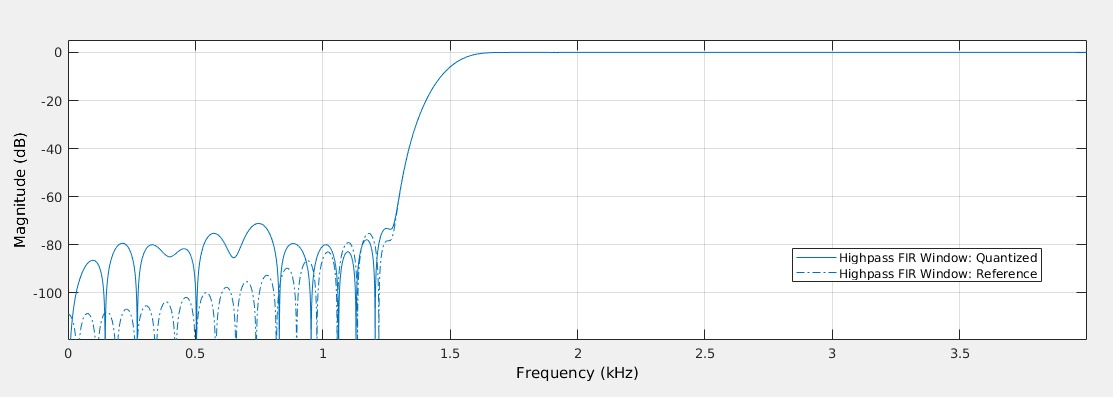
\includegraphics[width=0.80\textwidth]{firMatlab}\par\vspace{1cm}
    \clearpage
    \subsection{Code}

    \subsubsection{de main code.}
        
        \begin{lstlisting}[language=c]
#include <stdio.h>
#include <usbstk5505.h>
#include <usbstk5505_led.h>
#include <csl_intc.h>

#include "aic3204.h"
#include "fdacoefs.h"
#include "fir_buffer.h"

#define SAMPLES_PER_SECOND 8000 // possible values: 48000, 24000, 16000, 12000, 9600, and 8000
#define ADC_GAIN  0// range: 0dB to 48 dB
#define DAC_GAIN 0// range: -6dB to 29dB


extern void VECSTART(void);

FIRBuffer *buffer;
interrupt void I2S0receive() {

    fir_buffer_store_sample(buffer, AIC3204_readLeft());
    AIC3204_writeLeft(fir_buffer_output_sample(buffer, COEFFICIENTS));

}

int main(void) {
    buffer = fir_buffer_new(COEFFICIENTS_LENGTH);

    USBSTK5505_init();
    AIC3204_init(SAMPLES_PER_SECOND, ADC_GAIN, DAC_GAIN);
    IRQ_setVecs((Uint32)(&VECSTART));
    IRQ_plug(PROG1_EVENT,&I2S0receive);
    IRQ_enable(PROG1_EVENT);
    IRQ_globalEnable();

    while(1);
}
            \end{lstlisting}
            \clearpage	
        
            \subsubsection{De header van de fir buffer}
            \begin{lstlisting}[language=c]
#ifndef __FIR_BUFFER__
#define __FIR_BUFFER__

#include <csl_intc.h>

typedef struct {
    int size;
    Int16 *buffer;
    int currentBufferIndex;
} FIRBuffer;

FIRBuffer * fir_buffer_new(int size);
void fir_buffer_store_sample(FIRBuffer *buffer, Int16 sample);
Int16 fir_buffer_output_sample(FIRBuffer *buffer, const Int16 *coefficients);

#endif//__FIR_BUFFER__
        
            \end{lstlisting}
            \clearpage
        
            \subsubsection{Code van de fir buffer}
            \begin{lstlisting}[language=c]
#include <stdlib.h>
#include "fir_buffer.h";

FIRBuffer * fir_buffer_new(int size) {
    FIRBuffer *firBuffer = (FIRBuffer *)malloc(sizeof(FIRBuffer));
    //TODO: Still have to solve potential nullpointer issues.

    firBuffer->size = size;
    firBuffer->buffer = malloc(sizeof(Int16) * size);
    firBuffer->currentBufferIndex = 0;

    return firBuffer;
}

void fir_buffer_store_sample(FIRBuffer *buffer, Int16 sample) {
    buffer->currentBufferIndex += 1;

    if(buffer->currentBufferIndex == buffer->size) {
            buffer->currentBufferIndex = 0;
    }

    buffer->buffer[buffer->currentBufferIndex] = sample;
}

Int16 fir_buffer_output_sample(FIRBuffer *buffer, const Int16 *coefficients) {
    Int32 output = 0;
    int k;
    for(k = 0; k < buffer->size; k++){
        int bufferIndex = buffer->currentBufferIndex - k;
        if(bufferIndex < 0){
            bufferIndex += buffer->size;
        }
        output += (Int32)coefficients[k] * (Int32)buffer->buffer[bufferIndex];
    }

    return((Int16)(output >> 15));
}
            \end{lstlisting}
            \clearpage	
        
            \begin{lstlisting}[language=c]
/*
* Filter Coefficients (C Source) generated by the Filter Design and Analysis Tool
* Generated by MATLAB(R) 9.2 and the DSP System Toolbox 9.4.
* Generated on: 09-Oct-2017 11:48:44
*/

/*
* Discrete-Time FIR Filter (real)
* -------------------------------
* Filter Structure  : Direct-Form FIR
* Filter Length     : 101
* Stable            : Yes
* Linear Phase      : Yes (Type 1)
* Arithmetic        : single
*/
/*
* Warning - Filter coefficients were truncated to fit specified data type.  
*   The resulting response may not match generated theoretical response.
*   Use the Filter Design & Analysis Tool to design accurate
*   int16 filter coefficients.
*/
#include <csl_intc.h>
#define COEFFICIENTS_LENGTH 101

const Int16 COEFFICIENTS[COEFFICIENTS_LENGTH] = {
0,      0,      0,      1,      1,     -1,     -3,     -2,      4,
7,      0,    -12,    -12,      8,     25,     12,    -26,    -40,
0,     55,     49,    -31,    -94,    -41,     88,    131,      0,
-170,   -147,     90,    266,    115,   -238,   -350,      0,    443,
381,   -233,   -686,   -298,    626,    938,      0,  -1271,  -1159,
767,   2541,   1311,  -3664,  -9621,  20480,  -9621,  -3664,   1311,
2541,    767,  -1159,  -1271,      0,    938,    626,   -298,   -686,
-233,    381,    443,      0,   -350,   -238,    115,    266,     90,
-147,   -170,      0,    131,     88,    -41,    -94,    -31,     49,
55,      0,    -40,    -26,     12,     25,      8,    -12,    -12,
0,      7,      4,     -2,     -3,     -1,      1,      1,      0,
0,      0
};	
            \end{lstlisting}
            \clearpage
        
        
            \subsection{Het resultaat}
            \clearpage